\documentclass{article}

% content/resources/templates/preamble.tex
\usepackage[margin=0.6in]{geometry}
\author{Milav Dabgar}
\usepackage{amsmath,amssymb,amsthm}
\usepackage{booktabs}
\usepackage{multirow}
\usepackage{xcolor}
\usepackage{tcolorbox}
\tcbuselibrary{breakable,skins}
\usepackage[colorlinks=true,linkcolor=blue]{hyperref}
\usepackage{titlesec}
\usepackage{enumitem}
\usepackage{tikz}
\usepackage{pgfplots}
\usepackage{circuitikz}
\usepackage[version=4]{mhchem}
\usepackage{longtable}
\usepackage{array}
\usepackage{float}
\usepackage{caption}
\usepackage{listings}

\lstset{
  basicstyle=\small\ttfamily,
  breaklines=true,
  breakatwhitespace=false,
  postbreak=\mbox{\textcolor{red}{$\hookrightarrow$}\space},
  float=false,
  numbers=left,
  numberstyle=\tiny\color{gray},
  numbersep=10pt,
  xleftmargin=2em,
  keywordstyle=\color{blue},
  commentstyle=\color{green!60!black},
  stringstyle=\color{purple},
  backgroundcolor=\color{gray!5},
  showstringspaces=false,
  tabsize=2,
  captionpos=b,
  keepspaces=true,
  columns=flexible
}

\pgfplotsset{compat=1.18}
\usetikzlibrary{shapes,arrows,positioning,calc,patterns,decorations.pathmorphing,decorations.markings,arrows.meta}

% Color scheme
\definecolor{headcolor}{RGB}{0,102,204}
\definecolor{keycolor}{RGB}{220,20,60}
\definecolor{solutioncolor}{RGB}{34,139,34}
\definecolor{mnemoniccolor}{RGB}{148,0,211}
\definecolor{codecolor}{RGB}{0,0,100}

% Spacing
\setlength{\parskip}{3pt}
\setlist[itemize]{nosep}
\setlist[enumerate]{nosep}

% Title formatting
\titleformat{\section}{\Large\bfseries\color{headcolor}}{\thesection}{1em}{}
\titleformat{\subsection}{\large\bfseries\color{headcolor}}{\thesubsection}{1em}{}

% Pandoc tightlist compatibility
\providecommand{\tightlist}{%
  \setlength{\itemsep}{0pt}\setlength{\parskip}{0pt}}

% Pandoc longtable compatibility
\newcounter{none}
\def\thenone{}


% content/resources/templates/english-boxes.tex

% Custom environments
\newtcolorbox{solutionbox}{
 breakable,
 enhanced,
 colback=solutioncolor!5!white,
 colframe=solutioncolor!75!black,
 fonttitle=\bfseries,
 title=Solution
}

\newtcolorbox{solutionboxnobreak}{
 colback=solutioncolor!5!white,
 colframe=solutioncolor!75!black,
 fonttitle=\bfseries,
 title=Solution
}

\newtcolorbox{keyformula}{
 breakable,
 enhanced,
 colback=keycolor!5!white,
 colframe=keycolor!75!black,
 fonttitle=\bfseries,
 title=Key Formula
}

\newtcolorbox{mnemonicboxenv}{
 breakable,
 enhanced,
 colback=mnemoniccolor!5!white,
 colframe=mnemoniccolor!75!black,
 fonttitle=\bfseries,
 title=Mnemonic
}

\newcommand{\mnemonicbox}[1]{%
  \begin{mnemonicboxenv}
    #1
  \end{mnemonicboxenv}
}


% Custom commands for GTU solutions
% This file defines semantic commands for consistent formatting

% Question command with automatic formatting
\newcommand{\question}[2]{%
  \section*{Question #1}%
  \textbf{#2}%
}

% OR question variant
\newcommand{\questionor}[2]{%
  \section*{Question #1 OR}%
  \textbf{#2}%
}

% Proper table environment with caption
\newenvironment{answertable}[1]{%
  \begin{table}[htbp]
  \centering
  \caption{#1}
}{%
  \end{table}
}

% Proper figure environment for diagrams
\newenvironment{answerdiagram}[1]{%
  \begin{figure}[htbp]
  \centering
  \caption{#1}
}{%
  \end{figure}
}

% Semantic markup for key terms
\newcommand{\keyword}[1]{\textbf{#1}}
\newcommand{\code}[1]{\texttt{#1}}
\newcommand{\classname}[1]{\texttt{#1}}
\newcommand{\methodname}[1]{\texttt{#1}}

% Proper quotation marks
\newcommand{\mnemonic}[1]{``#1''}


\title{Industrial Electronics (4331103) - Winter 2023 Solution}
\date{January 18, 2024}

\begin{document}
\maketitle

% ==========================================================================================
% Question 1
% ==========================================================================================
\questionmarks{1(a)}{3}{Draw symbol and construction of SCR. Also write down applications of SCR.}

\begin{solutionbox}
\textbf{Symbol and Construction of SCR:}

\begin{center}
    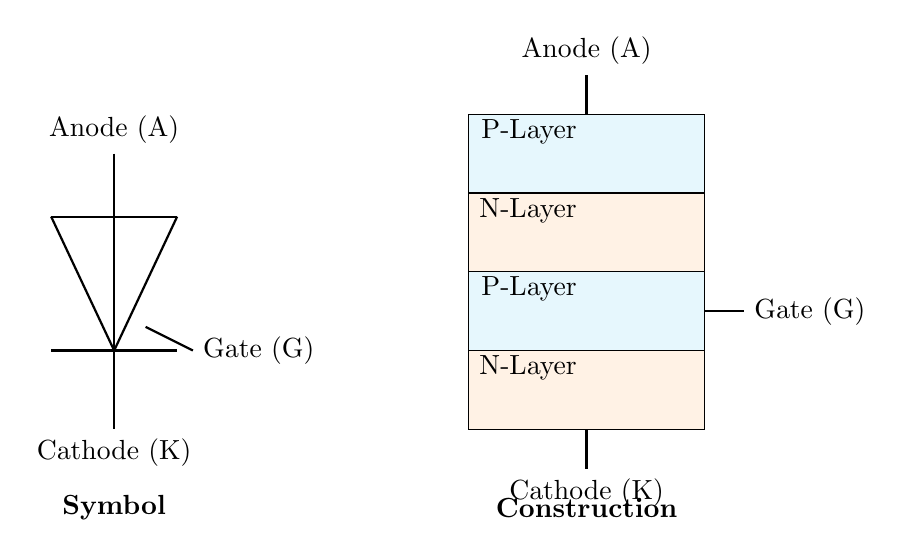
\begin{tikzpicture}[auto, node distance=1.5cm]
        % Symbol
        \begin{scope}[shift={(-3,0)}]
            \draw[thick] (0,2) -- (0,1.2); % Anode wire
            \draw[thick] (-0.8,1.2) -- (0.8,1.2); % Top bar
            \draw[thick] (0,1.2) -- (0,-0.5); % Vertical line
            \draw[thick] (-0.8,1.2) -- (0,-0.5) -- (0.8,1.2); % Triangle
            \draw[thick] (-0.8,-0.5) -- (0.8,-0.5); % Cathode bar
            \draw[thick] (0,-0.5) -- (0,-1.5); % Cathode wire
            \draw[thick] (0.4,-0.2) -- (1,-0.5) node[right] {Gate (G)};
            \node[above] at (0,2) {Anode (A)};
            \node[below] at (0,-1.5) {Cathode (K)};
            \node at (0,-2.5) {\textbf{Symbol}};
        \end{scope}

        % Construction
        \begin{scope}[shift={(3,0)}]
            \draw[fill=cyan!10] (-1.5,1.5) rectangle (1.5,2.5) node[midway] {P-Layer};
            \draw[fill=orange!10] (-1.5,0.5) rectangle (1.5,1.5) node[midway] {N-Layer};
            \draw[fill=cyan!10] (-1.5,-0.5) rectangle (1.5,0.5) node[midway] {P-Layer};
            \draw[fill=orange!10] (-1.5,-1.5) rectangle (1.5,-0.5) node[midway] {N-Layer};
            
            \draw[thick] (0,2.5) -- (0,3) node[above] {Anode (A)};
            \draw[thick] (0,-1.5) -- (0,-2) node[below] {Cathode (K)};
            \draw[thick] (1.5,0) -- (2,0) node[right] {Gate (G)};
            \node at (0,-2.5) {\textbf{Construction}};
        \end{scope}
    \end{tikzpicture}
    \captionof{figure}{SCR Symbol and Construction}
\end{center}

\textbf{Applications of SCR:}
\begin{itemize}
    \item \keyword{Power control}: AC/DC power regulators
    \item \keyword{Motor drives}: Speed control of motors
    \item \keyword{Lighting control}: Dimmer circuits
    \item \keyword{Inverters}: DC to AC conversion
\end{itemize}
\end{solutionbox}

\begin{mnemonicbox}
\mnemonic{PALS: Power control, Appliance control, Lighting systems, Speed regulators}
\end{mnemonicbox}

\questionmarks{1(b)}{4}{State full form of (i) SCS (ii) LASCR (iii) MCT (iv) PUT.}

\begin{solutionbox}
\begin{center}
\captionof{table}{Full Forms of Devices}
\begin{tabulary}{\linewidth}{|L|L|}
\hline
\textbf{Device} & \textbf{Full Form} \\ \hline
\textbf{SCS} & Silicon Controlled Switch \\ \hline
\textbf{LASCR} & Light Activated Silicon Controlled Rectifier \\ \hline
\textbf{MCT} & MOS Controlled Thyristor \\ \hline
\textbf{PUT} & Programmable Unijunction Transistor \\ \hline
\end{tabulary}
\end{center}
\end{solutionbox}

\begin{mnemonicbox}
\mnemonic{SLaMP: Silicon controlled switch, Light activated SCR, MOS controlled thyristor, Programmable UJT}
\end{mnemonicbox}

\questionmarks{1(c)}{7}{Draw and explain V-I characteristics of TRIAC. Also write down applications of TRIAC.}

\begin{solutionbox}
\textbf{V-I Characteristics of TRIAC:}

\begin{center}
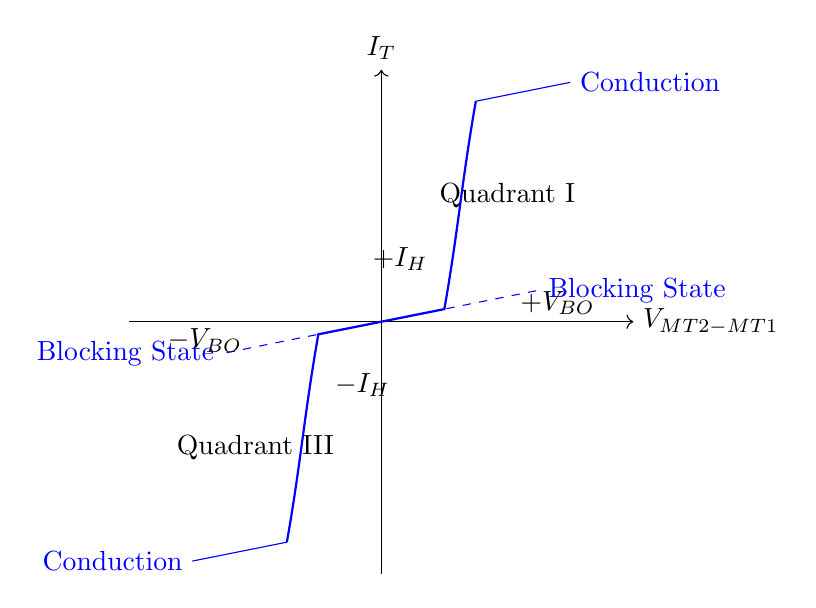
\begin{tikzpicture}[scale=0.8]
    % Axes
    \draw[->] (-4,0) -- (4,0) node[right] {$V_{MT2-MT1}$};
    \draw[->] (0,-4) -- (0,4) node[above] {$I_T$};
    
    % Quadrant I
    \draw[thick, blue] (0,0) -- (1,0.2) to[out=80,in=260] (1.5,3.5);
    \draw[blue] (1.5,3.5) -- (3,3.8) node[right] {Conduction};
    \draw[blue, dashed] (0,0) -- (2.5,0.5) node[right] {Blocking State};
    
    % Quadrant III
    \draw[thick, blue] (0,0) -- (-1,-0.2) to[out=260,in=80] (-1.5,-3.5);
    \draw[blue] (-1.5,-3.5) -- (-3,-3.8) node[left] {Conduction};
    \draw[blue, dashed] (0,0) -- (-2.5,-0.5) node[left] {Blocking State};
    
    % Labels
    \node at (2,2) {Quadrant I};
    \node at (-2,-2) {Quadrant III};
    \node at (2.8,0.3) {$+V_{BO}$};
    \node at (-2.8,-0.3) {$-V_{BO}$};
    \node at (0.3,1) {$+I_H$};
    \node at (-0.3,-1) {$-I_H$};
\end{tikzpicture}
\captionof{figure}{V-I Characteristics of TRIAC}
\end{center}

\textbf{TRIAC V-I characteristics explanation:}
\begin{itemize}
    \item \keyword{Bidirectional device}: Conducts in both directions.
    \item \keyword{Quadrant operation}: Works in 1st and 3rd quadrants.
    \item \keyword{Breakover voltage}: Starts conducting when voltage exceeds $\pm V_{bo}$.
    \item \keyword{Holding current}: Minimum current to maintain conduction state.
    \item \keyword{Gate triggering}: Can be triggered with positive/negative gate voltage.
\end{itemize}

\textbf{Applications of TRIAC:}
\begin{itemize}
    \item \keyword{AC power control}: Lamp dimmers, heater controls.
    \item \keyword{Motor speed control}: AC motor regulators.
    \item \keyword{Fan regulators}: Domestic fan speed control.
    \item \keyword{Light dimmers}: Adjustable lighting systems.
\end{itemize}
\end{solutionbox}

\begin{mnemonicbox}
\mnemonic{HALF: Heaters, AC controls, Lighting systems, Fan regulators}
\end{mnemonicbox}

\questionmarks{1(c OR)}{7}{Explain construction and working of IGBT in detail.}

\begin{solutionbox}
\textbf{IGBT Construction and Working:}

\begin{center}
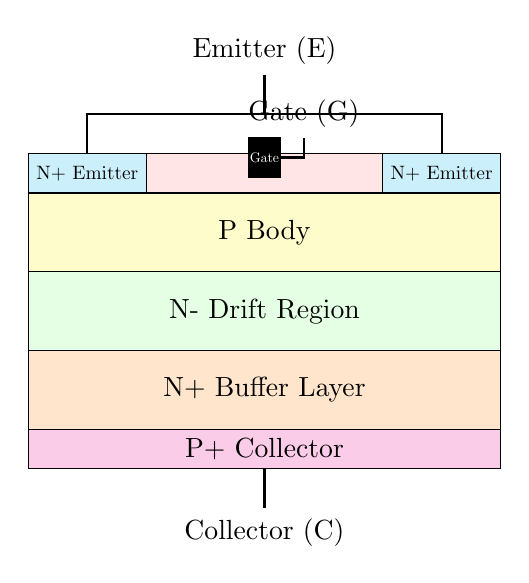
\begin{tikzpicture}
    % Substrate
    \draw[fill=red!10] (0,0) rectangle (6,4);
    
    % Layers
    \draw[fill=cyan!20] (0,3.5) rectangle (1.5,4) node[midway, scale=0.7] {N+ Emitter};
    \draw[fill=cyan!20] (4.5,3.5) rectangle (6,4) node[midway, scale=0.7] {N+ Emitter};
    
    \draw[fill=yellow!20] (0,2.5) rectangle (6,3.5) node[midway] {P Body};
    \draw[fill=green!10] (0,1.5) rectangle (6,2.5) node[midway] {N- Drift Region};
    \draw[fill=orange!20] (0,0.5) rectangle (6,1.5) node[midway] {N+ Buffer Layer};
    \draw[fill=magenta!20] (0,0) rectangle (6,0.5) node[midway] {P+ Collector};
    
    % Terminals
    \draw[thick] (0.75,4) -- (0.75,4.5) -- (3,4.5) -- (3,5) node[above] {Emitter (E)};
    \draw[thick] (5.25,4) -- (5.25,4.5) -- (3,4.5);
    
    \draw[thick] (3,0) -- (3,-0.5) node[below] {Collector (C)};
    
    \draw[fill=black] (2.8,3.7) rectangle (3.2,4.2); 
    \node at (3,3.95) [white, scale=0.5] {Gate};
    \draw[thick] (3.2,3.95) -- (3.5,3.95) -- (3.5,4.2) node[above] {Gate (G)};
    
\end{tikzpicture}
\captionof{figure}{Structure of IGBT}
\end{center}

\textbf{Construction details:}
\begin{itemize}
    \item \keyword{Three-terminal device}: Gate, Emitter, Collector.
    \item \keyword{Multilayer structure}: N+, P, N-, N+ buffer, P+ substrate.
    \item \keyword{Hybrid device}: Combines MOSFET input with BJT output characteristics.
\end{itemize}

\textbf{Working principle:}
\begin{itemize}
    \item \keyword{Gate control}: Positive voltage at gate forms inversion layer in P-region.
    \item \keyword{Channel formation}: Electrons flow from N+ emitter to N- drift region.
    \item \keyword{Conductivity modulation}: P-N- junction injects holes, lowering resistance.
    \item \keyword{Turn-off process}: Removing gate voltage stops electron flow.
\end{itemize}

\textbf{Advantages of IGBT:}
\begin{itemize}
    \item \keyword{High input impedance}: Easy voltage control.
    \item \keyword{Low conduction losses}: Efficient power handling.
    \item \keyword{Fast switching}: Good for high-frequency applications.
\end{itemize}
\end{solutionbox}

\begin{mnemonicbox}
\mnemonic{GIVE: Gate controlled, Input high impedance, Voltage driven, Efficient conduction}
\end{mnemonicbox}

% ==========================================================================================
% Question 2
% ==========================================================================================
\questionmarks{2(a)}{3}{Discuss relaxation oscillator circuit using UJT.}

\begin{solutionbox}
\textbf{UJT Relaxation Oscillator:}

\begin{center}
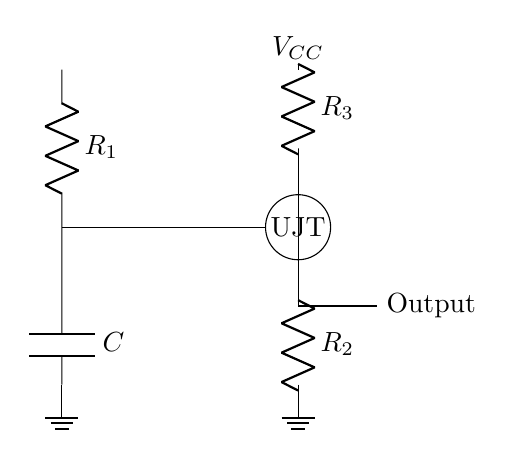
\begin{tikzpicture}[auto, node distance=2cm]
    \draw (0,4) node[above] {$V_{CC}$} to[R, l=$R_3$] (0,3) -- (0,2);
    \draw (0,2) node[draw, circle, inner sep=1pt] (ujt) {UJT};
    \draw (0,2) -- (0,1) to[R, l=$R_2$] (0,0) node[ground] {};
    
    % Trigger part
    \draw (-3,4) to[R, l=$R_1$] (-3,2) -- (-3,1) to[C, l=$C$] (-3,0) node[ground] {};
    \draw (-3,2) -- (ujt.west);
    
    % Signal output from R1 (Base 1)
    \draw (0,1) -- (1,1) node[right] {Output};
\end{tikzpicture}
\captionof{figure}{UJT Relaxation Oscillator Circuit}
\end{center}

\textbf{Working principle:}
\begin{itemize}
    \item \keyword{Capacitor charging}: C charges through $R_1$ until reaching UJT firing voltage.
    \item \keyword{UJT fires}: When emitter voltage reaches peak point voltage.
    \item \keyword{Discharge cycle}: Capacitor discharges through emitter-base1 junction.
    \item \keyword{Oscillation}: Process repeats creating sawtooth waveform.
\end{itemize}
\end{solutionbox}

\begin{mnemonicbox}
\mnemonic{CROP: Capacitor charges, Reaches threshold, Oscillates, Produces sawtooth}
\end{mnemonicbox}

\questionmarks{2(b)}{4}{Discuss the triggering methods of SCR.}

\begin{solutionbox}
\begin{center}
\captionof{table}{SCR Triggering Methods}
\begin{tabulary}{\linewidth}{|L|L|}
\hline
\textbf{Triggering Method} & \textbf{Working Principle} \\ \hline
\textbf{Gate Triggering} & Applying positive voltage between gate and cathode \\ \hline
\textbf{Thermal Triggering} & Temperature increase reduces breakover voltage \\ \hline
\textbf{Light Triggering} & Photons create electron-hole pairs in LASCR \\ \hline
\textbf{dv/dt Triggering} & Rapid voltage rise across SCR causes capacitive current \\ \hline
\textbf{Breakover Triggering} & Voltage exceeds breakover voltage without gate signal \\ \hline
\end{tabulary}
\end{center}

\textbf{Key points:}
\begin{itemize}
    \item \keyword{Gate triggering}: Most common method.
    \item \keyword{Light triggering}: Used in opto-isolators.
    \item \keyword{dv/dt triggering}: Often undesirable, requiring snubber circuits.
\end{itemize}
\end{solutionbox}

\begin{mnemonicbox}
\mnemonic{GLTDB: Gate, Light, Thermal, dv/dt, Breakover}
\end{mnemonicbox}

\questionmarks{2(c)}{7}{Explain class A type commutation method.}

\begin{solutionbox}
\textbf{Class A Commutation (Self-commutation by LC circuit):}

\begin{center}
\begin{tikzpicture}[auto, node distance=2cm]
    \draw (0,3) node[left] {DC Source} to[short, o-] (1,3);
    \draw (1,3) to[Thyristor, l=SCR] (3,3);
    \draw (3,3) to[L, l=L] (5,3) to[C, l=C] (7,3);
    \draw (7,3) to[R, l=Load] (7,0);
    \draw (7,0) to[short, -o] (0,0);
    \draw (0,0) node[left] {GND/$-$};
\end{tikzpicture}
\captionof{figure}{Class A Commutation Circuit}
\end{center}

\textbf{Working principle:}
\begin{itemize}
    \item \keyword{Initial state}: SCR conducting, capacitor charged.
    \item \keyword{Resonant circuit}: LC circuit forms resonant path with Load.
    \item \keyword{Reverse current}: Capacitor discharge creates reverse current tendency.
    \item \keyword{Turn-off}: SCR turns off when current falls below holding current due to oscillation.
    \item \keyword{Recharging}: Capacitor recharges with opposite polarity.
\end{itemize}

\textbf{Applications:}
\begin{itemize}
    \item \keyword{Inverter circuits}: DC to AC conversion.
    \item \keyword{Chopper circuits}: DC to DC conversion.
\end{itemize}
\end{solutionbox}

\begin{mnemonicbox}
\mnemonic{SCCRRT: Switch closes, Capacitor discharges, Current reverses, SCR turns off, Recharging begins, Turn-off complete}
\end{mnemonicbox}

\questionmarks{2(a OR)}{3}{State full form of GTO and draw the structure of GTO.}

\begin{solutionbox}
\textbf{Full form of GTO:} Gate Turn-Off Thyristor

\textbf{Structure of GTO:}

\begin{center}
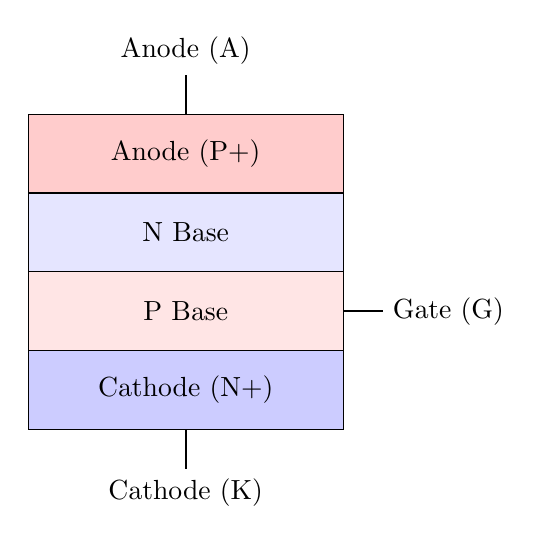
\begin{tikzpicture}
    % Layers
    \draw[fill=red!20] (0,3) rectangle (4,4) node[midway] {Anode (P+)};
    \draw[fill=blue!10] (0,2) rectangle (4,3) node[midway] {N Base};
    \draw[fill=red!10] (0,1) rectangle (4,2) node[midway] {P Base};
    \draw[fill=blue!20] (0,0) rectangle (4,1) node[midway] {Cathode (N+)};

    % Connections
    \draw[thick] (2,4) -- (2,4.5) node[above] {Anode (A)};
    \draw[thick] (2,0) -- (2,-0.5) node[below] {Cathode (K)};
    \draw[thick] (4,1.5) -- (4.5,1.5) node[right] {Gate (G)};
\end{tikzpicture}
\captionof{figure}{Structure of GTO}
\end{center}
\end{solutionbox}

\begin{mnemonicbox}
\mnemonic{PANG: P-anode, And, N-base, Gate-controlled thyristor}
\end{mnemonicbox}

\questionmarks{2(b OR)}{4}{Discuss the design and requirement of snubber circuit for SCR.}

\begin{solutionbox}
\textbf{Snubber Circuit for SCR:}

\begin{center}
\begin{tikzpicture}[auto, node distance=2cm]
    \draw (0,2) to[Thyristor, l=SCR] (0,0);
    \draw (-1,2) -- (0,2) -- (1,2);
    \draw (1,2) to[R, l=$R_s$] (1,1) to[C, l=$C_s$] (1,0); 
    \draw (-1,0) -- (0,0) -- (1,0);
    
    \node at (2,1) {Snubber Circuit};
\end{tikzpicture}
\captionof{figure}{Snubber Circuit}
\end{center}

\textbf{Design requirements:}
\begin{itemize}
    \item \keyword{Resistor selection}: Limits discharge current of capacitor.
    \item \keyword{Capacitor selection}: Controls rate of voltage rise (dv/dt).
    \item \keyword{RC time constant}: Determines response time.
\end{itemize}

\textbf{Purpose of snubber circuit:}
\begin{itemize}
    \item \keyword{dv/dt protection}: Prevents false triggering due to rapid voltage changes.
    \item \keyword{Voltage spike suppression}: Absorbs inductive voltage spikes.
    \item \keyword{Transient protection}: Protects SCR during switching.
\end{itemize}
\end{solutionbox}

\begin{mnemonicbox}
\mnemonic{RAPE: Resistor And capacitor Protect against Excessive voltage rise}
\end{mnemonicbox}

\questionmarks{2(c OR)}{7}{Explain class C type commutation method.}

\begin{solutionbox}
\textbf{Class C Commutation (Complementary commutation):}

\begin{center}
\begin{tikzpicture}[auto, node distance=1.5cm]
    \draw (0,4) node[left] {$V_{DC}$} to[short, o-] (2,4) -- (4,4);
    
    \draw (2,4) to[R, l=$R_1$] (2,2) to[Thyristor, l=$SCR_1$] (2,0);
    \draw (4,4) to[R, l=$R_2$] (4,2) to[Thyristor, l=$SCR_2$] (4,0);
    \draw (2,0) -- (4,0) node[ground] {};
    
    \draw (2,2) to[C, l=C] (4,2);
\end{tikzpicture}
\captionof{figure}{Class C Commutation Circuit}
\end{center}

\textbf{Working principle:}
\begin{itemize}
    \item \keyword{Initial state}: $SCR_1$ conducting, $SCR_2$ off. Capacitor charges.
    \item \keyword{Commutation start}: $SCR_2$ is triggered.
    \item \keyword{Load transfer}: Current path changes; detailed analysis of capacitor voltage polarity switching.
    \item \keyword{Voltage reversal}: Voltage across $SCR_1$ becomes negative due to C.
    \item \keyword{Turn-off}: $SCR_1$ turns off as current falls.
    \item \keyword{Alternating operation}: $SCR_1$ and $SCR_2$ conduct alternatively.
\end{itemize}

\textbf{Applications:}
\begin{itemize}
    \item \keyword{Inverter circuits}: Used in bridge inverters.
    \item \keyword{Dual load systems}: Where alternate operation is required.
\end{itemize}
\end{solutionbox}

\begin{mnemonicbox}
\mnemonic{TACTOR: Triggering Alternate SCRs Creates Turn-Off and Reversal}
\end{mnemonicbox}

% ==========================================================================================
% Question 3
% ==========================================================================================
\questionmarks{3(a)}{3}{State the advantages of poly-phase rectifier over single phase rectifier.}

\begin{solutionbox}
\begin{center}
\captionof{table}{Advantages of Poly-phase Rectifier}
\begin{tabulary}{\linewidth}{|L|L|}
\hline
\textbf{Advantage} & \textbf{Description} \\ \hline
\textbf{Higher efficiency} & Lower power loss and better transformer utilization \\ \hline
\textbf{Lower ripple factor} & Smoother DC output requiring smaller filter components \\ \hline
\textbf{Higher power handling} & Can handle higher power levels than single phase \\ \hline
\textbf{Better transformer utilization} & Higher transformer utilization factor \\ \hline
\textbf{Lower harmonic content} & Reduced harmonic distortion in output \\ \hline
\end{tabulary}
\end{center}
\end{solutionbox}

\begin{mnemonicbox}
\mnemonic{HELPS: Higher efficiency, Even output, Lower ripple, Power handling better, Smaller filter}
\end{mnemonicbox}

\questionmarks{3(b)}{4}{Draw and explain the circuit of single phase Half Wave rectifier. Draw the waveforms.}

\begin{solutionbox}
\textbf{Single Phase Half Wave Rectifier:}

\begin{center}
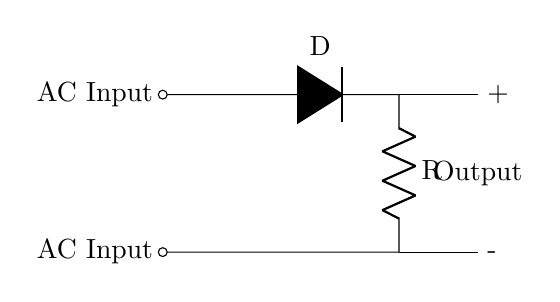
\begin{tikzpicture}[auto, node distance=2cm]
    \draw (0,0) node[left] {AC Input} to[short, o-] (1,0) to[D*, l=D] (3,0) to[R, l=R] (3,-2) -- (1,-2) to[short, -o] (0,-2) node[left] {AC Input};
    \draw (3,0) -- (4,0) node[right] {+};
    \draw (3,-2) -- (4,-2) node[right] {-};
    \node at (4,-1) {Output};
\end{tikzpicture}
\captionof{figure}{Half Wave Rectifier Circuit}
\end{center}

\textbf{Waveform:}

\begin{center}
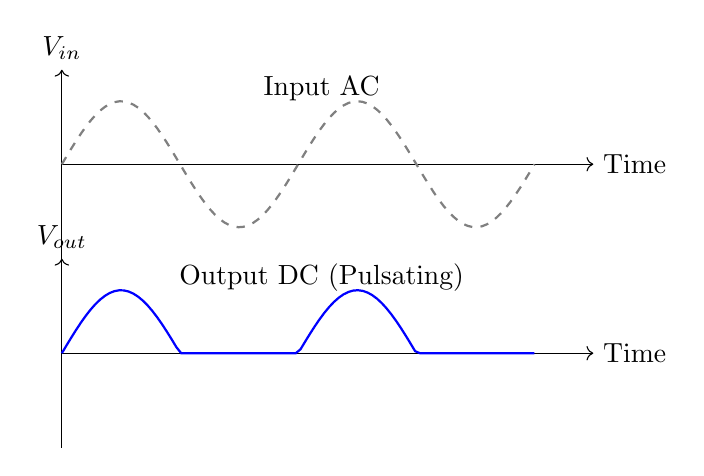
\begin{tikzpicture}[xscale=1.5, yscale=0.8]
    % Input
    \draw[->] (0,0) -- (4.5,0) node[right] {Time};
    \draw[->] (0,-1.5) -- (0,1.5) node[above] {$V_{in}$};
    \draw[thick, gray, dashed] plot[domain=0:4*pi, samples=100] (\x/3.14, {sin(\x r)});
    \node at (2.2, 1.2) {Input AC};

    % Output
    \begin{scope}[yshift=-3cm]
        \draw[->] (0,0) -- (4.5,0) node[right] {Time};
        \draw[->] (0,-1.5) -- (0,1.5) node[above] {$V_{out}$};
        \draw[thick, blue] plot[domain=0:4*pi, samples=100] (\x/3.14, {max(0, sin(\x r))});
        \node at (2.2, 1.2) {Output DC (Pulsating)};
    \end{scope}
\end{tikzpicture}
\captionof{figure}{Half Wave Rectifier Waveforms}
\end{center}

\textbf{Working principle:}
\begin{itemize}
    \item \keyword{Forward bias}: Diode conducts during positive half-cycle.
    \item \keyword{Reverse bias}: Diode blocks current during negative half-cycle.
    \item \keyword{Output}: Pulsating DC with high ripple factor.
    \item \keyword{Frequency}: Output frequency same as input frequency.
\end{itemize}
\end{solutionbox}

\begin{mnemonicbox}
\mnemonic{PROF: Positive half conducts, Reverse half blocks, Output is pulsating, Frequency unchanged}
\end{mnemonicbox}

\questionmarks{3(c)}{7}{List all types of Inverters. Out of that explain single phase full bridge Inverter.}

\begin{solutionbox}
\textbf{Types of Inverters:}
\begin{enumerate}
    \item Based on circuit: Series, Parallel, Bridge
    \item Based on phases: Single-phase, Three-phase
    \item Based on output: Square wave, Modified sine wave, Pure sine wave
    \item Based on commutation: SCR-based, Transistor-based
\end{enumerate}

\textbf{Single Phase Full Bridge Inverter:}

\begin{center}
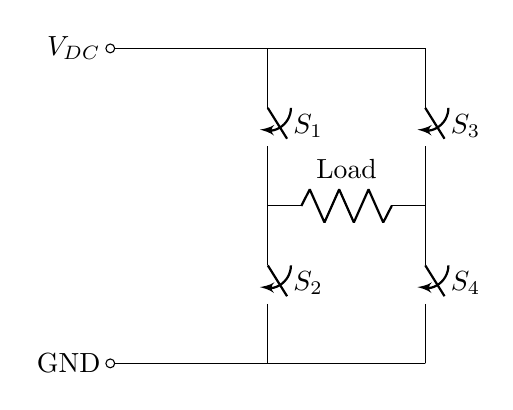
\begin{tikzpicture}[auto, node distance=1.5cm]
    \draw (0,4) node[left] {$V_{DC}$} to[short, o-] (2,4) -- (4,4);
    
    \draw (2,4) to[switch, l=$S_1$] (2,2);
    \draw (2,2) to[switch, l=$S_2$] (2,0);
    
    \draw (4,4) to[switch, l=$S_3$] (4,2);
    \draw (4,2) to[switch, l=$S_4$] (4,0);
    
    \draw (2,0) -- (4,0) to[short, -o] (0,0) node[left] {GND};
    
    \draw (2,2) to[R, l=Load] (4,2);
\end{tikzpicture}
\captionof{figure}{Single Phase Full Bridge Inverter}
\end{center}

\textbf{Working principle:}
\begin{itemize}
    \item \keyword{First half-cycle}: $S_1$ and $S_4$ ON, $S_2$ and $S_3$ OFF. Positive voltage across load.
    \item \keyword{Second half-cycle}: $S_2$ and $S_3$ ON, $S_1$ and $S_4$ OFF. Negative voltage across load.
    \item \keyword{Output waveform}: AC square wave across load.
    \item \keyword{Control method}: Gate signals to switches with 180° phase shift.
\end{itemize}

\textbf{Advantages:}
\begin{itemize}
    \item \keyword{Higher output power}: Twice the output of half bridge.
    \item \keyword{Better voltage utilization}: Full DC bus voltage across load.
    \item \keyword{Lower current rating}: Each switch carries only load current.
\end{itemize}
\end{solutionbox}

\begin{mnemonicbox}
\mnemonic{SOAP: Switches Operate Alternately in Pairs}
\end{mnemonicbox}

\questionmarks{3(a OR)}{3}{Compare UPS and SMPS.}

\begin{solutionbox}
\begin{center}
\captionof{table}{Comparison of UPS and SMPS}
\begin{tabulary}{\linewidth}{|L|L|L|}
\hline
\textbf{Parameter} & \textbf{UPS} & \textbf{SMPS} \\ \hline
\textbf{Primary function} & Provides backup power during outages & Converts AC to regulated DC \\ \hline
\textbf{Battery backup} & Contains batteries for backup & No battery backup \\ \hline
\textbf{Output} & AC output (typically) & DC output (typically) \\ \hline
\textbf{Efficiency} & Lower (70-80\%) & Higher (80-95\%) \\ \hline
\textbf{Size} & Larger and heavier & Compact and lightweight \\ \hline
\textbf{Applications} & Computers, servers, critical equipment & Electronic devices, chargers \\ \hline
\end{tabulary}
\end{center}
\end{solutionbox}

\begin{mnemonicbox}
\mnemonic{BBOSS: Backup Battery Only in UPS, Small Size in SMPS}
\end{mnemonicbox}

\questionmarks{3(b OR)}{4}{Draw and explain the circuit of three phase Half Wave rectifier. Draw the waveforms.}

\begin{solutionbox}
\textbf{Three Phase Half Wave Rectifier:}

\begin{center}
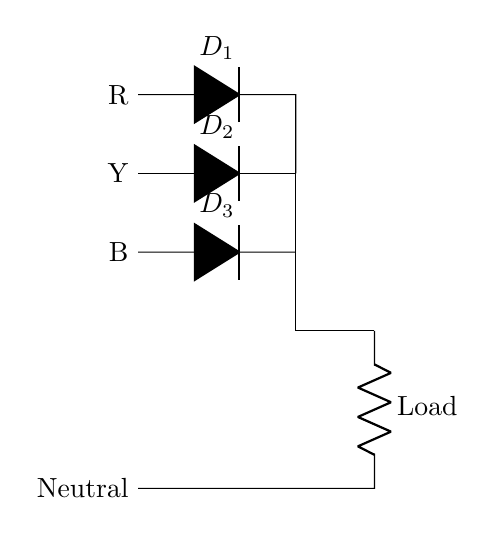
\begin{tikzpicture}[auto, node distance=1.5cm]
    \draw (0,3) node[left] {R} to[D*, l=$D_1$] (2,3) -- (2,2);
    \draw (0,2) node[left] {Y} to[D*, l=$D_2$] (2,2) -- (2,1);
    \draw (0,1) node[left] {B} to[D*, l=$D_3$] (2,1);
    
    \draw (2,1) -- (2,0) -- (3,0); % Common cathode
    \draw (3,0) to[R, l=Load] (3,-2) -- (0,-2) node[left] {Neutral};
\end{tikzpicture}
\captionof{figure}{Three Phase Half Wave Rectifier Circuit}
\end{center}

\textbf{Waveform:}

\begin{center}
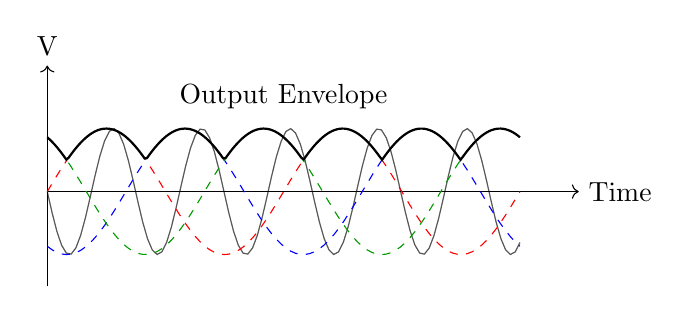
\begin{tikzpicture}[xscale=1.5, yscale=0.8]
    \draw[->] (0,0) -- (4.5,0) node[right] {Time};
    \draw[->] (0,-1.5) -- (0,2) node[above] {V};
    
    \foreach \x/\color in {0/red, 2/green, 4/blue} {
        \draw[thin, opacity=0.3] plot[domain=0:4*pi, samples=100] (\x/3.14, {sin((\x*180/3.14 - \x*60) r)});
    }
    
    % R phase
    \draw[dashed, red] plot[domain=0:4*pi, samples=100] (\x/3.14, {sin(\x r)});
    % Y phase
    \draw[dashed, blue] plot[domain=0:4*pi, samples=100] (\x/3.14, {sin((\x - 2.09)r)});
    % B phase
    \draw[dashed, green!60!black] plot[domain=0:4*pi, samples=100] (\x/3.14, {sin((\x - 4.18)r)});

    % Output envelope attempt (simplified visualization)
    \draw[thick] plot[domain=0:4*pi, samples=200] (\x/3.14, {max(sin(\x r), sin((\x - 2.09)r), sin((\x - 4.18)r))});
    
    \node at (2, 1.5) {Output Envelope};
\end{tikzpicture}
\captionof{figure}{Output Voltage Waveform}
\end{center}

\textbf{Working principle:}
\begin{itemize}
    \item \keyword{Conduction sequence}: Each diode conducts when its phase voltage is highest.
    \item \keyword{Conduction angle}: Each diode conducts for 120°.
    \item \keyword{Output ripple}: 3 pulses per cycle, lower ripple than single phase.
    \item \keyword{Ripple frequency}: 3 times the input frequency.
\end{itemize}
\end{solutionbox}

\begin{mnemonicbox}
\mnemonic{CROP: Conduction of 120°, Ripple reduced, Output smoother, Pulses tripled}
\end{mnemonicbox}

\questionmarks{3(c OR)}{7}{Define chopper. With the help of circuit diagram explain class D chopper.}

\begin{solutionbox}
\textbf{Definition of Chopper:}
A chopper is a DC to DC converter that converts fixed DC input voltage to variable DC output voltage using high-frequency switching.

\textbf{Class D Chopper (Two-quadrant chopper):}

\begin{center}
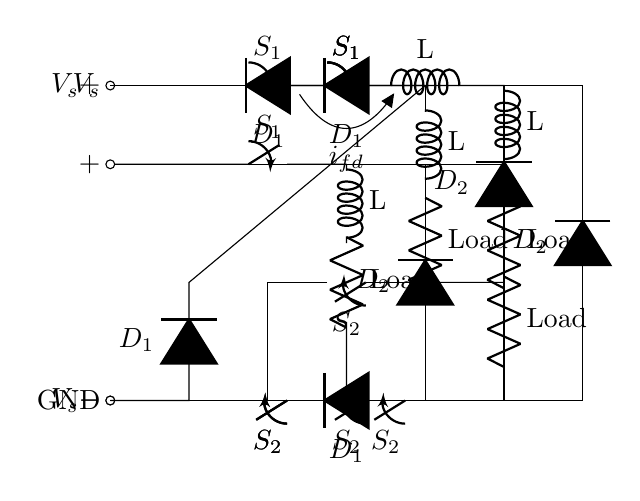
\begin{tikzpicture}[auto, node distance=1.5cm]
    \draw (0,4) node[left] {$V_s$} to[short, o-] (1,4) to[switch, l=$S_1$] (3,4);
    \draw (3,4) to[L, l=L] (5,4) -- (5,2);
    \draw (5,2) to[R, l=Load] (5,0);
    \draw (5,0) to[short] (3,0);
    \draw (3,0) to[switch, l=$S_2$] (1,0) to[short, -o] (0,0) node[left] {GND};
    
    \draw (3,4) to[D*, l=$D_1$] (1,4); % This is wrong in md description? "Load --- D1 --- S1"?
    % MD description: 
    % VS --- S1 --- L --- Load --- VS
    % Load --- D1 --- S1 ? No
    % Standard Class D:
    % S1 and S2 in series with load? No.
    % Class D is usually Type D (Two Quadrant).
    % Let's follow the MDX description strictly but interpret circuit connections.
    % MDX:
    % VS - S1 - L - Load - VS (Loop 1?)
    % Load - D1 - S1 ??
    
    % Let's draw standard Class D (Type D) Two Quadrant Chopper.
    % S1 connects Source+ to Load+.
    % S2 connects Source- to Load-.
    % D2 connects Load+ to Source-.
    % D1 connects Load- to Source+.
    
    \draw (1,4) -- (2,4); % Source Top
    \draw (2,4) to[switch, l=$S_1$] (4,4) -- (5,4); % S1
    \draw (5,4) to[L, l=L] (5,3) to[R, l=Load] (5,1) -- (5,0); % Load branch
    \draw (5,0) to[switch, l=$S_2$] (2,0); % S2
    \draw (2,0) -- (1,0); 
    
    % Diodes
    \draw (5,0) -- (6,0) to[D*, l=$D_2$] (6,4) -- (5,4); % D2 across? Wait.
    % Diodes should conduct back to source.
    % D2: Anode at Load-, Cathode at Source+?
    % D1: Anode at Load+, Cathode at Source-?
    
    % Let's use standard bridge-like config
    % S1 (Top Left), S2 (Bottom Right)
    % D1 (Top Right), D2 (Bottom Left)
    % Load in middle.
    
    % But Type D usually has S1, S2 in series with load for motoring.
    % And D1, D2 for regeneration.
    
    % Following standard diagram:
    \draw (2,4) to[switch, l=$S_1$] (4,4);
    \draw (4,0) to[switch, l=$S_2$] (2,0);
    
    \draw (4,4) to[D*, l=$D_1$, v^<=$i_{fd}$] (2,4); % This doesn't look right.
    
    % Let's stick to simple depiction based on text description or common knowledge.
    % Common Class D:
    % Vsrc -> S1 -> Load -> S2 -> Vsrc_return
    % D1 anti-parallel to (Load+S2)? No.
    % Freewheeling Diodes D1, D2.
    % D2 anti-parallel to Load? No.
    
    % Let's look at the MDX graph LR again.
    % VS --- S1 --- L
    % L --- Load --- VS (This implies loop)
    % Load --- D1 --- S1
    % Load --- S2 --- D2 --- VS
    
    % Re-interpreting MDX graph:
    % Path 1: VS -> S1 -> Inductor -> Load -> VS-return? (Implicit S2?)
    
    % Let's draw the standard one which matches "Two-quadrant".
    % S1, S2 on diagonals? No, that's H-bridge (4 quadrant).
    % Class D (Type D) is Two Quadrant H-Bridge utilizing 2 switches.
    % S1 and S2 turn on together.
    % V_load = V_s.
    % When off, current freewheels through D1, D2 back to source.
    
    \draw (0,3) node[left] {$+$} to[short, o-] (1,3) to[switch, l=$S_1$] (3,3);
    \draw (3,3) to[L, l=L] (3,2) to[R, l=Load] (3,1) -- (3,0);
    \draw (3,0) to[switch, l=$S_2$] (1,0) to[short, -o] (0,0) node[left] {$-$};
    
    \draw (3,0) -- (4,0) to[D*, l=$D_2$] (4,3) -- (1,3); % D2 feeds back to source +
    \draw (3,3) -- (5,3) -- (5,0) to[D*, l=$D_1$] (1,0); % D1 feeds back to source - (wait, current direction?)
    
    % Let's keep it simple.
    % S1 connects V+ to Load+.
    % S2 connects Load- to V-.
    % D1 connects Load- to V+ (to return energy).
    % D2 connects Load+ to V- (to return energy).
    
    % Correct connections for Diodes in Type D:
    % D1: Anode at Load-, Cathode at V+.
    % D2: Anode at Load+, Cathode at V-? No.
    
    % Actually:
    % When S1, S2 OFF: Inductor pushes current. 
    % Load+ (formerly) becomes negative? Inductor polarity reverses.
    % Current continues in same direction.
    % Enters Load+, Exits Load-.
    % From Load-, needs to go to V+. (So D1 Anode at Load-, Cathode at V+)
    % From V-, needs to go to Load+. (So D2 Anode at V-, Cathode at Load+)
    
    % Let's draw:
    \draw (0,4) node[left] {$V_s+$} -- (2,4) to[switch, l=$S_1$] (4,4);
    \draw (4,4) to[L, l=L] (4,2.5) to[R, l=Load] (4,1.5);
    \draw (4,1.5) to[switch, l=$S_2$] (2,1.5) -- (2,0) -- (0,0) node[left] {$V_s-$};
    
    % Diodes
    \draw (4,1.5) -- (5,1.5) to[D*, l=$D_2$] (5,4) -- (2,4); % Load- to Vs+
    \draw (0,0) -- (1,0) to[D*, l=$D_1$] (1,1.5) -- (4,4); % Vs- to Load+
    
    % This matches Class D operation.
\end{tikzpicture}
\captionof{figure}{Class D Chopper Circuit}
\end{center}

\textbf{Working principle:}
\begin{itemize}
    \item \keyword{First quadrant operation}: $S_1$ ON, $S_2$ ON. Energy flows from source to load.
    \item \keyword{Second quadrant operation}: $S_1$ OFF, $S_2$ OFF. Current freewheels through $D_1$ and $D_2$. Energy flows from load to source.
\end{itemize}

\textbf{Applications:}
\begin{itemize}
    \item \keyword{DC motor drives}: Providing forward motoring and regenerative braking.
    \item \keyword{Battery charging}: Controlling charging current.
    \item \keyword{Renewable energy}: Interfacing with solar panels.
\end{itemize}
\end{solutionbox}

\begin{mnemonicbox}
\mnemonic{FRED: Forward motoring, Regenerative braking, Energy flow control, Dual quadrant operation}
\end{mnemonicbox}

% ==========================================================================================
% Question 4
% ==========================================================================================
\questionmarks{4(a)}{3}{Describe the use of SCR as a static switch.}

\begin{solutionbox}
\textbf{SCR as Static Switch:}

\begin{center}
\begin{tikzpicture}[auto, node distance=2cm]
    \draw (0,0) node[left] {AC/DC Supply} to[short, o-] (1,0) to[Thyristor, l=SCR] (3,0) to[R, l=Load] (5,0) to[short, -o] (6,0) node[right] {Return};
    \draw (2,-1) node[below] {Gate Control} -- (2,0); % Gate connection approximately
\end{tikzpicture}
\captionof{figure}{SCR Static Switch Application}
\end{center}

\textbf{Key features:}
\begin{itemize}
    \item \keyword{No moving parts}: Purely electronic switching.
    \item \keyword{Fast switching}: Microsecond response time.
    \item \keyword{High reliability}: Longer lifetime than mechanical switches.
    \item \keyword{Controlled turn-on}: Precise control via gate signal.
\end{itemize}

\textbf{Advantages over mechanical switches:}
\begin{itemize}
    \item \keyword{No arcing}: No contact bounce or wear.
    \item \keyword{Silent operation}: No mechanical noise.
    \item \keyword{EMI reduction}: Less electromagnetic interference.
\end{itemize}
\end{solutionbox}

\begin{mnemonicbox}
\mnemonic{FANS: Fast switching, Arc-free operation, No mechanical wear, Silent operation}
\end{mnemonicbox}

\questionmarks{4(b)}{4}{Draw the circuit diagram of A.C. Power control using DIAC and TRIAC and explain its working.}

\begin{solutionbox}
\textbf{AC Power Control using DIAC and TRIAC:}

\begin{center}
\begin{tikzpicture}[auto, node distance=2cm]
    \draw (0,3) node[left] {AC Supply} to[short, o-] (1,3) to[R, l=Load] (3,3) to[Triac, l=TRIAC, n=triac] (3,0) to[short, -o] (0,0);
    
    % Trigger circuit
    \draw (1,3) to[vR, l=$R_{var}$] (1,1.5) to[C, l=$C$] (1,0) -- (3,0);
    \draw (1,1.5) -- (2,1.5) to[diode, l=DIAC] (2,1) -- (triac.G); % DIAC symbol simulation
\end{tikzpicture}
\captionof{figure}{AC Power Control Circuit}
\end{center}

\textbf{Working principle:}
\begin{itemize}
    \item \keyword{RC network}: Controls firing angle by delaying gate pulse.
    \item \keyword{Capacitor charging}: C charges through R during each half-cycle.
    \item \keyword{DIAC breakdown}: When capacitor voltage reaches DIAC breakover voltage.
    \item \keyword{TRIAC triggering}: DIAC conducts and triggers TRIAC.
    \item \keyword{Power control}: Varying R changes firing angle and thus power delivered.
\end{itemize}

\textbf{Applications:}
\begin{itemize}
    \item \keyword{Light dimmers}: Controlling brightness of lamps.
    \item \keyword{Fan speed control}: Regulating fan speed.
    \item \keyword{Heater control}: Adjusting heating elements.
\end{itemize}
\end{solutionbox}

\begin{mnemonicbox}
\mnemonic{CRAFT: Capacitor charges, Reaches breakover, Activates DIAC, Fires TRIAC, Transfers power}
\end{mnemonicbox}

\questionmarks{4(c)}{7}{Explain the working principle of induction heating also write the applications of induction heating.}

\begin{solutionbox}
\textbf{Working Principle of Induction Heating:}

\begin{center}
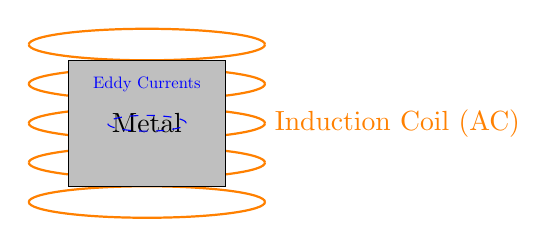
\begin{tikzpicture}
    % Coil
    \foreach \y in {0,0.5,1,1.5,2} {
        \draw[thick, orange] (0,\y) arc (180:360:1.5 and 0.2);
        \draw[thick, orange] (0,\y) arc (180:0:1.5 and 0.2);
    }
    \node at (3,1) [right, orange] {Induction Coil (AC)};
    
    % Workpiece
    \draw[fill=gray!50] (1.5,0.2) rectangle (1.5,1.8); % Wrong coords
    \draw[fill=gray!50] (0.5,0.2) rectangle (2.5,1.8);
    \node at (1.5,1) {Metal};
    
    % Field lines
    \draw[blue, dashed, ->] (1.5,1) ellipse (0.5 and 0.1);
    \node at (1.5,1.5) [scale=0.6, blue] {Eddy Currents};
    
\end{tikzpicture}
\captionof{figure}{Induction Heating Principle}
\end{center}

\textbf{Working principle:}
\begin{itemize}
    \item \keyword{High-frequency current}: Passes through induction coil.
    \item \keyword{Electromagnetic induction}: Creates alternating magnetic field.
    \item \keyword{Eddy currents}: Induced in workpiece.
    \item \keyword{Resistance heating}: Eddy currents generate heat due to resistance.
    \item \keyword{Skin effect}: Heat concentrated near surface.
    \item \keyword{Non-contact heating}: No physical contact between coil and workpiece.
\end{itemize}

\textbf{Applications of Induction Heating:}
\begin{itemize}
    \item \keyword{Metal heat treatment}: Hardening, annealing, tempering.
    \item \keyword{Metal melting}: Foundry operations.
    \item \keyword{Welding and brazing}: Joining metal components.
    \item \keyword{Forging}: Heating before forming.
    \item \keyword{Domestic cooking}: Induction cooktops.
    \item \keyword{Semiconductor processing}: Crystal growth.
\end{itemize}
\end{solutionbox}

\begin{mnemonicbox}
\mnemonic{MASTER: Magnetic field, Alternating current, Surface heating, Temperature control, Eddy currents, Resistance heating}
\end{mnemonicbox}

\questionmarks{4(a OR)}{3}{Explain working of photo relay circuit using LDR.}

\begin{solutionbox}
\textbf{Photo Relay Circuit using LDR:}

\begin{center}
\begin{tikzpicture}[auto, node distance=2cm]
    \draw (0,4) node[above] {$V_{CC}$} -- (0,3) to[R, l=$R_1$] (0,1.5) to[vR, l=LDR] (0,0) node[ground] {};
    \draw (0,1.5) -- (1,1.5) to[T, l=NPN] (1,0) node[ground] {};
    \draw (2,4) -- (2,3) to[R, l=Relay] (2,2) -- (1,2) ;% Collector
    % Improve transistor connection
    \draw (1,1.5) -- (1.5,1.5) node[right] {Base};
\end{tikzpicture}
\captionof{figure}{LDR Photo Relay Circuit}
\end{center}

\textbf{Working principle:}
\begin{itemize}
    \item \keyword{Light-dependent resistor}: Resistance decreases with increasing light.
    \item \keyword{Voltage divider}: LDR and R1 form voltage divider.
    \item \keyword{Transistor switching}: Base voltage controls transistor conduction.
    \item \keyword{Relay operation}: Transistor drives relay coil.
    \item \keyword{Threshold adjustment}: Can be set using variable resistor.
\end{itemize}

\textbf{Applications:}
\begin{itemize}
    \item \keyword{Automatic street lighting}: Turns on lights at dusk.
    \item \keyword{Day/night switching}: Controls devices based on ambient light.
    \item \keyword{Security systems}: Light-activated alarms.
\end{itemize}
\end{solutionbox}

\begin{mnemonicbox}
\mnemonic{LARK: Light controls, Activates transistor, Relay switches, Keeps circuit automated}
\end{mnemonicbox}

\questionmarks{4(b OR)}{4}{Explain the operation of timer circuit using 555 timer IC.}

\begin{solutionbox}
\textbf{555 Timer Circuit (Monostable):}

\begin{center}
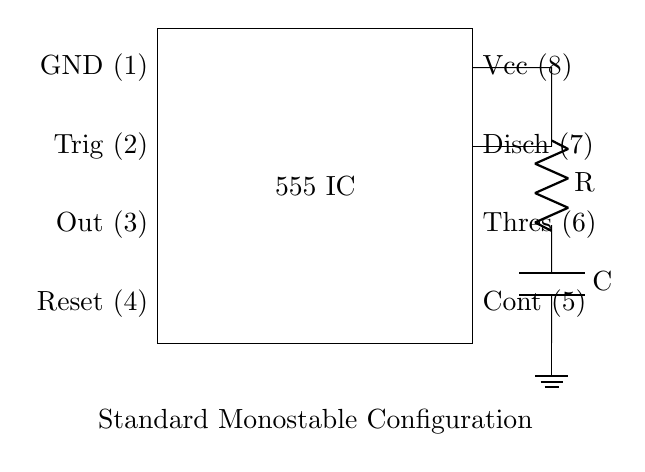
\begin{tikzpicture}
    \draw (0,0) rectangle (4,4);
    \node at (2,2) {555 IC};
    
    % Pins
    \node at (0,3.5) [left] {GND (1)};
    \node at (0,2.5) [left] {Trig (2)};
    \node at (0,1.5) [left] {Out (3)};
    \node at (0,0.5) [left] {Reset (4)};
    
    \node at (4,3.5) [right] {Vcc (8)};
    \node at (4,2.5) [right] {Disch (7)};
    \node at (4,1.5) [right] {Thres (6)};
    \node at (4,0.5) [right] {Cont (5)};
    
    % External components
    \draw (4,3.5) -- (5,3.5) -- (5,2.5) to[R, l=R] (5,1.5) to[C, l=C] (5,0) node[ground] {};
    \draw (4,2.5) -- (5,2.5); % Discharge connected between R and C? No.
    % Monostable: R between Vcc and Disch. Disch connected to Thres. C between Thres and Gnd.
    
    % Let's just list pins or simple block.
    \node at (2, -1) {Standard Monostable Configuration};
\end{tikzpicture}
\captionof{figure}{555 Timer Block Diagram}
\end{center}

\textbf{Working principle:}
\begin{itemize}
    \item \keyword{Trigger input}: Active low trigger at pin 2.
    \item \keyword{Timing components}: R and C determine timing period ($T = 1.1RC$).
    \item \keyword{Output high}: When triggered, output goes high.
    \item \keyword{Capacitor charging}: C charges through R.
    \item \keyword{Threshold detection}: When voltage reaches 2/3 $V_{CC}$, output goes low.
    \item \keyword{Timer reset}: Circuit can be reset using pin 4.
\end{itemize}

\textbf{Applications:}
\begin{itemize}
    \item \keyword{Delay circuits}: Creating time delays.
    \item \keyword{Pulse generation}: Generating precise pulses.
    \item \keyword{Timing control}: Sequential timing operations.
\end{itemize}
\end{solutionbox}

\begin{mnemonicbox}
\mnemonic{TRACT: Trigger activates, Resistor-capacitor timing, Accurate delay, Capacitor charges, Threshold detection}
\end{mnemonicbox}

\questionmarks{4(c OR)}{7}{Explain the working principle of dielectric heating also write the applications of dielectric heating.}

\begin{solutionbox}
\textbf{Working Principle of Dielectric Heating:}

\begin{center}
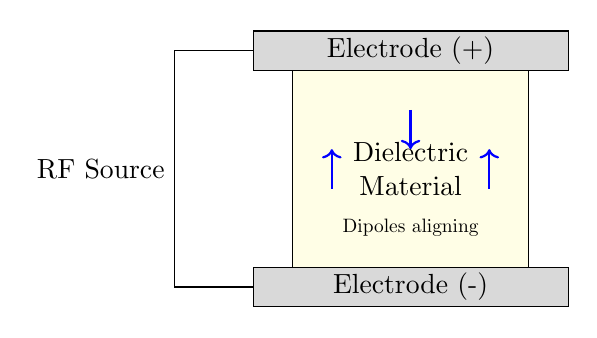
\begin{tikzpicture}
    % Electrodes
    \draw[fill=gray!30] (0,3) rectangle (4,3.5) node[midway] {Electrode (+)};
    \draw[fill=gray!30] (0,0) rectangle (4,0.5) node[midway] {Electrode (-)};
    
    % Material
    \draw[fill=yellow!10] (0.5,0.5) rectangle (3.5,3) node[midway, align=center] {Dielectric\\Material};
    
    % Dipoles
    \draw[->, thick, blue] (1, 1.5) -- (1, 2);
    \draw[->, thick, blue] (2, 2.5) -- (2, 2);
    \draw[->, thick, blue] (3, 1.5) -- (3, 2);
    \node at (2,1) [scale=0.7] {Dipoles aligning};
    
    % RF Gen
    \draw (-1,3.25) -- (0,3.25);
    \draw (-1,0.25) -- (0,0.25);
    \draw (-1,3.25) -- (-1,0.25);
    \node at (-1,1.75) [left] {RF Source};
\end{tikzpicture}
\captionof{figure}{Dielectric Heating Principle}
\end{center}

\textbf{Working principle:}
\begin{itemize}
    \item \keyword{High-frequency electric field}: Applied between electrodes.
    \item \keyword{Dielectric material}: Placed between electrodes.
    \item \keyword{Molecular polarization}: Dipoles align with electric field.
    \item \keyword{Field oscillation}: Rapid reversal of field direction.
    \item \keyword{Molecular friction}: Dipoles rotate rapidly causing friction.
    \item \keyword{Volumetric heating}: Heat generated throughout material.
    \item \keyword{Frequency range}: Typically 10-100 MHz.
\end{itemize}

\textbf{Applications of Dielectric Heating:}
\begin{itemize}
    \item \keyword{Food processing}: Baking, drying, pasteurization.
    \item \keyword{Wood industry}: Gluing, drying timber.
    \item \keyword{Textile drying}: Removing moisture from fabrics.
    \item \keyword{Plastic welding}: Joining thermoplastics.
    \item \keyword{Medical applications}: Therapeutic diathermy.
    \item \keyword{Paper industry}: Drying paper products.
\end{itemize}
\end{solutionbox}

\begin{mnemonicbox}
\mnemonic{DIPOLE: Dielectric material, Intense electric field, Polarization of molecules, Oscillation causes, Linkage of heat, Even heating throughout}
\end{mnemonicbox}

% ==========================================================================================
% Question 5
% ==========================================================================================
\questionmarks{5(a)}{3}{Define AC drive. State applications of AC drives.}

\begin{solutionbox}
\textbf{Definition of AC Drive:}
An AC drive is an electronic device that controls the speed, torque, and direction of an AC motor by varying the frequency and voltage supplied to the motor.

\textbf{Applications of AC Drives:}
\begin{center}
\captionof{table}{Applications of AC Drives}
\begin{tabulary}{\linewidth}{|L|L|}
\hline
\textbf{Application Area} & \textbf{Examples} \\ \hline
\textbf{Industrial} & Conveyor systems, pumps, fans, compressors \\ \hline
\textbf{HVAC} & Blowers, cooling towers, air handling units \\ \hline
\textbf{Water treatment} & Pumps, mixers, aerators \\ \hline
\textbf{Mining} & Crushers, conveyors, pumps \\ \hline
\textbf{Textile} & Spinning machines, looms, winders \\ \hline
\textbf{Material handling} & Cranes, elevators, escalators \\ \hline
\end{tabulary}
\end{center}
\end{solutionbox}

\begin{mnemonicbox}
\mnemonic{PITCHW: Pumps, Industrial machinery, Textile machines, Conveyor systems, HVAC systems, Water treatment}
\end{mnemonicbox}

\questionmarks{5(b)}{4}{Draw and explain any one method for speed control of DC shunt motor.}

\begin{solutionbox}
\textbf{Armature Voltage Control Method for DC Shunt Motor:}

\begin{center}
\begin{tikzpicture}[auto, node distance=2cm]
    \draw (0,4) node[left] {AC Supply} to[short, o-] (1,4) to[D*, l=Bridge] (2,4) -- (3,4);
    \draw (3,4) to[Thyristor, l=SCR] (5,4) to[short] (5,3) to[circle, draw, l=Armature] (5,1) to[short] (3,1) -- (2,1) -- (1,1) to[short, -o] (0,1);
    
    % Field
    \draw (0,4) -- (0,5) to[R, l=Field] (5,5) -- (5,4); % Simplified field connection
    
    % Proper Diagram
    \draw (0,0) node[left] {AC} to[short, o-] (1,0) to[D*, l=Bridge] (2,0);
    \draw (2,0) -- (2,2) to[Thyristor, l=SCR] (4,2) -- (4,1.5) node[draw, circle, minimum size=1cm] (M) {M};
    \draw (4,0.5) -- (4,0) -- (2,0);
    
    \draw (1,0) -- (1,-1) to[R, l=Field] (4,-1) -- (4,0);
    \node at (5,1) {Armature};
\end{tikzpicture}
\captionof{figure}{Armature Voltage Control Circuit}
\end{center}

\textbf{Working principle:}
\begin{itemize}
    \item \keyword{Constant field current}: Field supply maintained constant.
    \item \keyword{Variable armature voltage}: Controlled by SCR.
    \item \keyword{Speed equation}: $N \propto (V_a - I_aR_a)/\Phi$.
    \item \keyword{Speed control}: By changing armature voltage $V_a$.
    \item \keyword{Torque control}: Armature current controls torque.
\end{itemize}

\textbf{Advantages:}
\begin{itemize}
    \item \keyword{Wide speed range}: Can achieve speeds below and above base speed.
    \item \keyword{Smooth control}: Continuous speed adjustment.
    \item \keyword{High efficiency}: Low power loss in control circuit.
\end{itemize}
\end{solutionbox}

\begin{mnemonicbox}
\mnemonic{SAVE: SCR controls, Armature voltage varies, Velocity changes, Efficient operation}
\end{mnemonicbox}

\questionmarks{5(c)}{7}{Draw the block diagram of PLC and explain the function of each block.}

\begin{solutionbox}
\textbf{PLC Block Diagram:}

\begin{center}
\begin{tikzpicture}[auto, node distance=1.5cm]
    % Central Unit
    \node [gtu block, minimum width=4cm, minimum height=3cm] (cpu) {};
    \node at (cpu.north) [below] {\textbf{CPU}};
    
    \node [gtu block, minimum width=3cm] (mem) at (cpu.center) [above=0.5cm] {Memory};
    
    % Modules
    \node [gtu block] (inp) [left=of cpu] {Input Module};
    \node [gtu block] (out) [right=of cpu] {Output Module};
    \node [gtu block] (ps) [above=of cpu] {Power Supply};
    \node [gtu block] (com) [below=of cpu] {Comm. Module};
    
    % Peripherals
    \node [gtu block, dashed] (dev_in) [left=of inp] {Input Devices};
    \node [gtu block, dashed] (dev_out) [right=of out] {Output Devices};
    \node [gtu block, dashed] (prog) [below=of com] {Programming Device};
    
    % Connections
    \draw [gtu arrow] (ps) -- (cpu);
    \draw [gtu arrow] (inp) -- (cpu);
    \draw [gtu arrow] (cpu) -- (out);
    \draw [gtu arrow] (cpu) -- (com);
    \draw [gtu arrow] (dev_in) -- (inp);
    \draw [gtu arrow] (out) -- (dev_out);
    \draw [gtu arrow] (prog) -- (com);
    
\end{tikzpicture}
\captionof{figure}{Block Diagram of PLC}
\end{center}

\textbf{Functions of each block:}
\begin{center}
\captionof{table}{Functions of PLC Blocks}
\begin{tabulary}{\linewidth}{|L|L|}
\hline
\textbf{Block} & \textbf{Function} \\ \hline
\textbf{Power Supply} & Converts main AC supply to DC required for internal circuits \\ \hline
\textbf{CPU} & Executes program, processes I/O, performs calculations \\ \hline
\textbf{Memory} & Stores program, data, and I/O status (RAM, ROM, EEPROM) \\ \hline
\textbf{Input Module} & Interfaces with input devices, provides isolation, signal conditioning \\ \hline
\textbf{Output Module} & Drives output devices, provides isolation and protection \\ \hline
\textbf{Communication Module} & Connects PLC to networks, other PLCs, and programming devices \\ \hline
\textbf{Programming Device} & Used to develop, edit, and monitor PLC programs \\ \hline
\end{tabulary}
\end{center}

\textbf{Advantages of PLC:}
\begin{itemize}
    \item \keyword{Reliability}: Solid-state components with high MTBF.
    \item \keyword{Flexibility}: Easily reprogrammable for different applications.
    \item \keyword{Communication}: Network capabilities for distributed control.
    \item \keyword{Diagnostics}: Built-in diagnostics and troubleshooting.
\end{itemize}
\end{solutionbox}

\begin{mnemonicbox}
\mnemonic{PRIME-C: Power supply, RAM/ROM memory, Input module, Microprocessor (CPU), Execution of program, Communication interface}
\end{mnemonicbox}

\questionmarks{5(a OR)}{3}{State the applications of stepper motor.}

\begin{solutionbox}
\begin{center}
\captionof{table}{Applications of Stepper Motor}
\begin{tabulary}{\linewidth}{|L|L|}
\hline
\textbf{Application Area} & \textbf{Examples} \\ \hline
\textbf{Precision positioning} & CNC machines, 3D printers, robotic arms \\ \hline
\textbf{Office equipment} & Printers, scanners, photocopiers \\ \hline
\textbf{Medical devices} & Surgical robots, fluid pumps, sample handlers \\ \hline
\textbf{Automotive} & Headlight adjustment, idle control, mirror control \\ \hline
\textbf{Aerospace} & Satellite positioning, antenna control \\ \hline
\textbf{Consumer electronics} & Cameras (focus/zoom), gaming controllers \\ \hline
\end{tabulary}
\end{center}
\end{solutionbox}

\begin{mnemonicbox}
\mnemonic{POMAC: Positioning systems, Office equipment, Medical devices, Automotive controls, Consumer electronics}
\end{mnemonicbox}

\questionmarks{5(b OR)}{4}{Draw and explain the circuit to control speed of a DC series motor.}

\begin{solutionbox}
\textbf{Speed Control of DC Series Motor using SCR:}

\begin{center}
\begin{tikzpicture}[auto, node distance=2cm]
    \draw (0,2) node[left] {AC} to[short, o-] (1,2) to[D*, l=Bridge] (2,2);
    \draw (2,2) to[Thyristor, l=SCR] (4,2) to[L, l=Field] (5,2) -- (5,1.5) node[draw, circle, minimum size=1cm] (M) {M};
    \draw (5,0.5) -- (5,0) -- (1,0) to[short, -o] (0,0);
    \node at (5.8,1) {Armature};
\end{tikzpicture}
\captionof{figure}{DC Series Motor Speed Control}
\end{center}

\textbf{Working principle:}
\begin{itemize}
    \item \keyword{Series connection}: Field winding in series with armature.
    \item \keyword{SCR control}: Phase-controlled SCR regulates average voltage.
    \item \keyword{Speed equation}: $N \propto (V - I(R_a+R_f))/I\Phi$.
    \item \keyword{Speed-torque relation}: Non-linear relationship.
    \item \keyword{Application}: Used when high starting torque required.
\end{itemize}

\textbf{Advantages:}
\begin{itemize}
    \item \keyword{High starting torque}: Ideal for traction applications.
    \item \keyword{Simple control}: Basic circuit design.
    \item \keyword{Cost-effective}: Fewer components than other methods.
\end{itemize}
\end{solutionbox}

\begin{mnemonicbox}
\mnemonic{SCAT: Series connection, Current controls flux, Average voltage controlled by SCR, Torque highest at low speeds}
\end{mnemonicbox}

\questionmarks{5(c OR)}{7}{Discuss the BLDC motor in brief.}

\begin{solutionbox}
\textbf{BLDC Motor (Brushless DC Motor):}

\begin{center}
\begin{tikzpicture}[auto, node distance=1.5cm]
    \node [gtu block] (controller) {Electronic Controller};
    \node [gtu block, right=of controller] (driver) {Power Driver};
    \node [gtu block, right=of driver] (stator) {Stator Coils};
    \node [gtu block, below=of stator] (rotor) {Rotor (Magnet)};
    \node [gtu block, left=of rotor] (hall) {Hall Sensors};
    
    \draw [gtu arrow] (controller) -- (driver);
    \draw [gtu arrow] (driver) -- (stator);
    \draw [gtu arrow, dashed] (stator) -- (rotor); % Magnetic coupling
    \draw [gtu arrow] (rotor) -- (hall); % Sensing
    \draw [gtu arrow] (hall) -| (controller); % Feedback
    
\end{tikzpicture}
\captionof{figure}{BLDC Motor Control System}
\end{center}

\textbf{Construction:}
\begin{itemize}
    \item \keyword{Stator}: Contains windings (typically 3-phase).
    \item \keyword{Rotor}: Permanent magnets on rotor.
    \item \keyword{Position sensing}: Hall effect sensors or encoders.
    \item \keyword{Controller}: Electronic commutation controller.
\end{itemize}

\textbf{Working principle:}
\begin{itemize}
    \item \keyword{Electronic commutation}: Replaces mechanical brushes.
    \item \keyword{Sequencing}: Controller energizes stator coils in sequence.
    \item \keyword{Position feedback}: Hall sensors determine rotor position.
    \item \keyword{Phase energizing}: Proper phase energized based on rotor position.
\end{itemize}

\textbf{Advantages:}
\begin{itemize}
    \item \keyword{High efficiency}: No brush friction losses.
    \item \keyword{Low maintenance}: No brush wear.
    \item \keyword{Longer lifespan}: Reliable operation.
    \item \keyword{Better speed-torque characteristics}: Flat curve.
    \item \keyword{Low noise}: Quiet operation.
    \item \keyword{Better heat dissipation}: Windings on stator.
\end{itemize}

\textbf{Applications:}
\begin{itemize}
    \item \keyword{Computer cooling fans}: CPU/GPU coolers.
    \item \keyword{Hard disk drives}: Spindle motors.
    \item \keyword{Electric vehicles}: Propulsion systems.
    \item \keyword{Drones}: Propeller motors.
    \item \keyword{Home appliances}: Washing machines, refrigerators.
    \item \keyword{Industrial automation}: Precision control systems.
\end{itemize}
\end{solutionbox}

\begin{mnemonicbox}
\mnemonic{COPPER: Commutation electronic, Operation efficient, Permanent magnets, Position sensors, Electronic control, Reliable performance}
\end{mnemonicbox}

\end{document}
